Let  the intercept points be
\begin{align}
{\vec{P}}=\myvec{
  a\\
  0}
 , {\vec{Q}}=\myvec{
  0\\
  b}
  \text{ and }
   {\vec{R}}=\myvec{
  2\\
  2}
\end{align}
be the given point.  
Forming the collinearity matrix from 
		\eqref{prop:lin-dep-rank},
\begin{align}
	\myvec{ \vec{P}-\vec{Q} &\vec{P}-\vec{R}} 
	=
	 \myvec{
  a & a-2\\
  -b & -2
 }
\end{align}
which is singular if 
\begin{align}
 ab -2\brak{a+b} = 0
 \implies ab = 18
		\label{eq:11/10/2/13-a+b}
		\\
\because  a + b = 9.
\end{align}
$\therefore a,b$
are the roots of
\begin{align}
	x^2 -9x +18 = 0.
\end{align}
yielding
\begin{align}
	\myvec{a \\ b} = \myvec{6 \\ 3}, \myvec{3\\6}
\end{align}
Since 
\begin{align}
	\vec{m} = \myvec{a \\ -b},
	\vec{n} = \myvec{b \\ a} \equiv \myvec{1 \\ 2}, \myvec{2\\1}
\end{align}
Thus, the possible equations of the line are 
\begin{align}
\myvec{1 & 2}\vec{x} = 6
	\\
	\myvec{2&1}\vec{x} = 6
\end{align}
		See \figref{fig:11/10/2/13}.
	\begin{figure}[H]
		\centering
 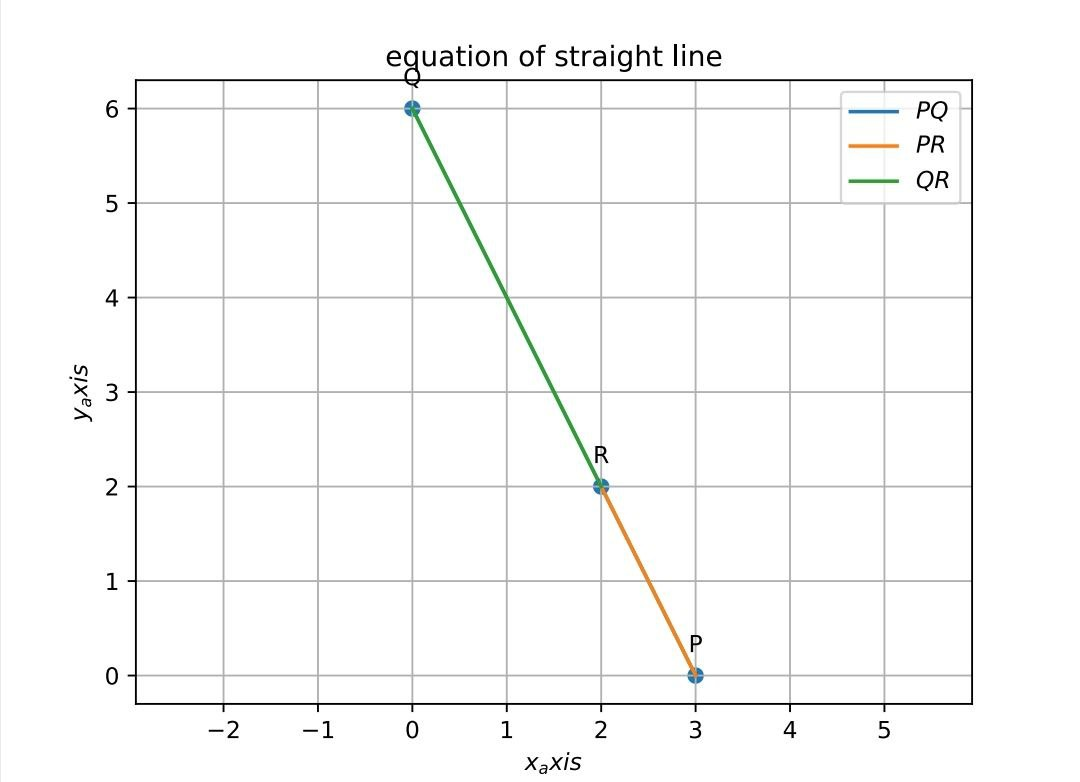
\includegraphics[width=0.75\columnwidth]{chapters/11/10/2/13/figs/assign4.png}
		\caption{}
		\label{fig:11/10/2/13}
  	\end{figure}
